\section{Materials and methods}\label{methodology}
This section explains the methodology and the optimization model developed in this work. After an introduction into the model in Section \ref{met:intro}, a detailed description of the mathematical formulation is presented in Section \ref{met:formulas}. The case study and scenario description comprise Section \ref{met:empirical}. The model validation is described in Section \ref{met:validate}, followed by the open-source programming environment in Section \ref{met:os}

\subsection{Introduction into the model}\label{met:intro}
In general, three agents are considered in the model with the following characteristics:
\paragraph{Governance} The governance's main objective is to decarbonize the residential heating sector. Therefore, the policy is to trigger a heating system change to a sustainable alternative on the multi-apartment building level through financial support for both property owner and tenants. The avowed aim is to find a cost-minimal and socially balanced solution. The financial support for the property owner can be realized either or both by an investment grant (paid directly from the governance) and adjusted rent-charge-related revenues (paid from the tenants). The tenants, for their part, can be financially supported directly by the governance through heating costs subsidy payments. 
\paragraph{Property owner} The property owner of the multi-apartment building provides the heating system for the tenants, and is profit-oriented. Thus, a heating system change toward a sustainable alternative is only realized in case of the economic viability of an investment. In this context, the property owner can achieve profitability of the alternative heating system by receiving an investment grant (to reduce the overnight investment costs) from the governance and a rent-charge-related revenue cash flow (from the tenants). 
\paragraph{Tenant} The tenant rents a dwelling/unit within the multi-apartment building from the property owner and has rent-related and energy-related spendings. The tenant cannot change the heating system on its authority but depends on the property owner's willingness to invest into a sustainable alternative. In connection with the existing heating system, the tenant's costs are increasing in consideration of CO\textsubscript{2} emissions and associated CO\textsubscript{2} prices. Nevertheless, the tenant aims to limit total costs in case of a heating system change at the level of the initial condition.\vspace{0.5cm}

Figure \ref{fig:methodology} shows a sketch illustrating the interrelations between the governance, the property owner, and the tenants. The governance can support the property owner financially by investment grants and by the permission of rent charge adjustments. At the same time, tenants are supported by a heating cost subsidy payment. The gray bar in the middle indicates that these financial benefits need to be socially balanced and overcome the differences in ownership within the multi-apartment building. The rent or rent charge adjustment is the direct financial exchange between the property owner and the tenant.\vspace{0.5cm}

\begin{figure}[h]
	\centering
	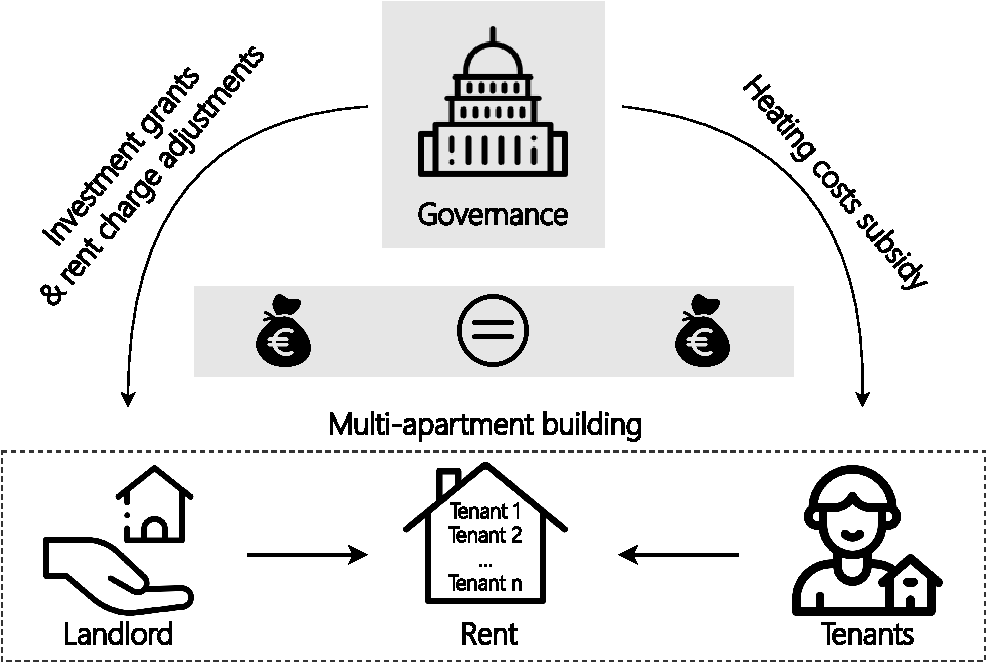
\includegraphics[width=0.7\linewidth]{figures/3_Methodology/Sketch.pdf}
	\caption{Sketch of the model illustrating the interrelations between the governance, property owner, and tenants. Financial support from the governance is socially balanced at the partly renovated multi-apartment rental building.}
	\label{fig:methodology}
\end{figure}

\subsection{Mathematical formulation of the model}\label{met:formulas}
This section explains the mathematical formulation of the optimization model in detail. First, the objective function is defined. Then, a detailed explanation of the model's constraints is given. 

\subsubsection{Model's objective function}
The objective function of the model is to minimize governance's total costs, including investment grants and subsidy payments\footnote{This corresponds to the maximization of the governance's net present value.}. Therefore, the objective function can be written as follows: 
\begin{align}\label{objective}
\underset{x}{\mathrm{min~}} \Psi + \sum_{y} \sum_{m} \frac{n}{(1+i_g)^y} \cdot \Omega_{y,m}
\end{align}

where $\Psi$ is the investment grant paid to the property owner and $\Omega_{y,m}$ is the heating costs subsidy payment paid to a single tenant in year $y$ and month $m$. In addition, $n$ is the number of tenants\footnote{It is assumed that the multi-apartment building consists of $n$ equal tenants/units.} and $i_g$ the governance's interest rate. The model's decision variables are included in the decision variable vector $x$. We refer to the nomenclature at the beginning of the paper containing a list of all decision variables.

\subsubsection{Model's constraints}
Equation \ref{c:demand} describes the load satisfaction of the total heat demand within the multi-apartment building using the alternative heating system in each time step (year and month) 
\begin{align}\label{c:demand}
n \cdot d_{y,m} \leq q_{y,m} \quad :\forall y,m
\end{align}

where $d_{y,m}$ is the total heat demand of a tenant's dwelling and $q_{y,m}$ the heat demand covered by the alternative heating system in $y$ and $m$. Building on this, Equation \ref{c:capacity} defines the minimum required newly installed capacity of the heating system alternative
\begin{align}\label{c:capacity}
\alpha_{m} \cdot q_{y,m} \leq \pi \quad :\forall y,m
\end{align}

where $\alpha_{m}$ is the load factor transforming the monthly amount of heat demand to the corresponding peak demand. Equation \ref{c:investment} defines the property owner's overnight investment costs ($\zeta$)
\begin{align}\label{c:investment}
\zeta = \pi \cdot c_{alt} + n \cdot c_{con} - \Psi
\end{align}

where $c_{alt}$ is the specific investment costs of the heating system alternative and $c_{con}$ the construction costs to adapt one dwelling/unit. Equation \ref{c:upper_inv_limit} defines the upper bound for the investment grant 
\begin{align}\label{c:upper_inv_limit}
\Psi \leq \hat{d} \cdot c_{alt} + n \cdot c_{con}
\end{align}

where $\hat{d}$ is the peak value of the heat demand. Equation \ref{c:revenues} defines the rent-related revenues of the property owner ($\lambda_{y,m}$)
\begin{align}\label{c:revenues}
\lambda_{y,m} = a \cdot n \cdot r_{y,m} \quad :\forall y,m
\end{align}

where $\bar{r}$ is the initial rent price, $r_{y,m}$ is the rent charge adjustment associated with the heating system change in $y$ and $m$ and $a$ are the areas of a tenant's dwelling. Equation \ref{c:npv} sets the property owner's net present value of the alternative heating system investment equal to 0
\begin{align}\label{c:npv}
-\zeta + \sum_{y} \sum_{m} \frac{1}{(1+i_l)^y} \cdot \lambda_{y,m} = 0
\end{align}

where $i_l$ is the property owner's interest rate. Equation \ref{c:ten1} defines the initial annual spendings of all tenants ($\kappa_{y}$) using the existing heating system 
\begin{align}\label{c:ten1}
\kappa_{y} = n \cdot (\bar{r} \cdot a + \sum_{m} q_{load,y,m} \cdot p_{init,y,m}) \quad :y=y_0
\end{align}

where $p_{init,y,m}$ is the price of the conventional fuel initially supplying the heat demand in $y$ and $m$. Building on this, Equation \ref{c:ten2} sets the tenants' total spendings ($K_{init}$)
\begin{align}\label{c:ten2}
K_{init} = -\sum_{y} \frac{1}{(1+i_{t})^y} \cdot \kappa_{y_0}
\end{align}

where $\sigma_{y_0}$ represents the initial tenants' spendings from Equation \ref{c:ten1} above, and $i_t$ the tenant's interest rate. Equation \ref{c:ten3} defines the total spendings of all tenants ($K_{alt}$) in case of implementing the sustainable heating system alternative.
\begin{align}\label{c:ten3}
	K_{alt} = -\sum_{y} \sum_{m} \frac{n}{(1+i_{t})^y} \left(a \cdot (\bar{r} + r_{y,m}) + q_{y,m} \cdot p_{alt,y,m}-\Omega_{y,m} \right)
\end{align}

Equation \ref{c:ten4} defines constant remaining spendings (i.e., economic viability) for the tenants in case of a heating system change.
\begin{align}\label{c:ten4}
K_{alt} = K_{init}
\end{align}

Equation \ref{c:con_sub} defines constant heating costs subsidy payments and Equation \ref{c:con_rent} is the constant total rent price for a tenant in $y$.
\begin{alignat}{2}
\Omega_{y,m} = \Omega_{y,m-1} \quad &:y\label{c:con_sub}\\
\bar{r} + r_{y,m} = \bar{r} + r_{y,m-1} \quad &:y\label{c:con_rent}
\end{alignat}

Equation \ref{c:temp_rent} allows rent charge adjustments by the property owner only every two years and Equations \ref{c:rent_upper1} and \ref{c:rent_upper2} set an upper bound to the rent charge adjustment
\begin{alignat}{3}
\bar{r} + r_{y,m} = \bar{r} + r_{y-1,m} \quad &:\forall y\backslash \{y_0\},m~\text{if}~y~\text{mod}~2=0\label{c:temp_rent}\\
\bar{r}+r_{y,m} \leq \rho \cdot \bar{r} \quad &:\forall y \in {y_0}\label{c:rent_upper1}\\
\bar{r}+r_{y,m} \leq \rho \cdot \left(\bar{r}+r_{y-1,m}\right) \quad &:\forall y\backslash \{y_0\}\label{c:rent_upper2}
\end{alignat}

by introducing $\rho$ as the rent charge adjustment upper bound. Equation \ref{c:final} defines the financial support parity between the property owner and all tenants at the multi-apartment building level from the governance's perspective 
\begin{align}\label{c:final}
\underbrace{\Psi +  n \cdot \sum_{y} \sum_{m} \frac{r_{y,m}}{(1+i_{g})^y}}_{\text{property owner financial support}}= \underbrace{n \cdot \sum_{y} \sum_{m} \frac{\Omega_{y,m}}{(1+i_{g})^y}}_{\text{tenants financial support}}
\end{align}

\subsection{Definition of the case study, scenarios, and empirical settings}\label{met:empirical}
\subsubsection{Multi-apartment building}
The model proposed in this work is applied to a typical multi-apartment building in an urban area. In particular, a partially renovated and natural gas-fired heating system in an old building in Vienna, Austria, is investigated. In $2020$, more than \SI{440000}{} natural gas-based heated dwellings existed in Vienna, Austria (\SI{48.5}{\%} of the total building stock) \cite{statistikaustriaheizen}. Nevertheless, this case study is representative for the European multi-apartment building stock in densely populated areas, as similar proportions of natural gas-fired heating systems exist in the residential heating sector there as well\footnote{For example, there are more than \SI{600000}{} natural gas-based systems covering residential heat demand in dwellings in Berlin, Germany, in $2020$ \cite{BDEW2019}.}.\vspace{0.5cm}

It is assumed that the multi-apartment building (including all dwellings) are privately owned by the property owner. The number of dwellings is $30$, whereby the area and rent price for each unit is equal. Each dwelling is rented by a tenant and heated by an individual natural gas-based heating system. The decarbonization of the existing heating systems can be realized by two different options, namely, a connection to the district heating network or the installation of an air-sourced heat pump\footnote{In general, it is assumed that the heat pump can be installed in the basement of the building. Nevertheless, the installation on the rooftop may also be considered. However, this explicit distinction is out of the scope of this work and is not further examined.}. It is assumed, that only one of the two technology alternatives is realized for all the dwellings. We refer to the empirical scaling and data in Section \ref{sec:data} for a detailed quantitative description of the multi-apartment building. 

\subsubsection{Scenarios}\label{sec:scenarios}
Four different quantitative scenarios are studied with the tailor-made model presented above. Input settings of three of them have been developed in the Horizon $2020$ research project openENTRANCE (\url{https://openentrance.eu/}) and describe a future European energy system development assuming to achieve the \SI{1.5}{\degreeCelsius} or \SI{2.0}{\degreeCelsius} climate target. These three scenarios are called \textit{Directed Transition} (DT), \textit{Societal Commitment} (SC), and \textit{Gradual Development} (GD) scenario\footnote{The openENTRANCE scenario \textit{Techno-Friendly} is not part of this work.}. The first two scenarios consider the remaining CO\textsubscript{2} budget of the \SI{1.5}{\degreeCelsius} climate target. Below, we briefly summarize the three openENTRANCE scenarios used in this work and refer to a detailed description to the studies in \cite{auer2020development} and \cite{auer2020quantitative}. For the reader with a particular interest in the openENTRANCE scenarios, we refer to the work in \cite{auer2019quantitative} in which the underlying storylines outlining the narrative frames of the quantitative scenarios can be found.\vspace{0.5cm}

The DT scenario leads to limiting the global temperature increase to \SI{1.5}{\degreeCelsius}. This is achieved by a breakthrough of new sustainable technologies triggered through strong policy incentives. The markets themselves do not push this development sufficiently and deliver weak financial impulses for the clean energy transition only. Besides, society is also too passive in supporting to achieve the ambitious \SI{1.5}{\degreeCelsius} target. Thus, in this work, it is assumed that the multi-apartment building is connected to the district heating network to reflect the strong policy driven character of implementing an alternative sustainable heating system. In the DT scenario, the CO\text{2} price rising from \SI{196}{EUR \per tCO_{2}} (in 2025) to \SI{680}{EUR \per tCO_{2}} (in 2040) results in a deep decarbonization of the European electricity and the heating sector, which is achieved in $2040$.\vspace{0.5cm}

The SC scenario also leads to limiting the global temperature increase to \SI{1.5}{\degreeCelsius}. In contrast to the previous scenario, decentralization of the energy system and active participation as well as societal acceptance of energy transition pushes sustainable development. In addition, currently existing clean technologies are significantly supported by policy incentives to foster its accelerated rollout. Thus, the SC scenario assumes deep decarbonization of the energy system without fundamental breakthroughs of novel technologies. Therefore, the multi-apartment building implements an air-sourced heat pump as a sustainable heating system alternative. A CO\text{2} price increase from \SI{62}{EUR \per tCO_{2}} (in 2025) to \SI{497}{EUR \per tCO_{2}} (in 2040) achieves deep decarbonization of the European electricity and heating sector in the SC scenario by $2040$.\vspace{0.5cm}

The GD scenario aims at achieving a global temperature increase of \SI{2.0}{\degreeCelsius}. In general, this describes a more conservative expression of a European energy system transition. This scenario includes a little of each of the ingredients of the remaining openENTRANCE scenarios: reduced policy incentives, limited social acceptance, and less promising technological advances. Both heating system alternatives (district heating connection and air-sourced heat pump installation) are examined in this work. The CO\text{2} price in the GD scenario is between \SI{83}{EUR \per tCO_{2}} (in 2025) and \SI{261}{EUR \per tCO_{2}} (in 2040). Deep decarbonization of the European electricity and heating sector is achieved in $2050$.\vspace{0.5cm}

In addition to the three openENTRANCE scenarios, the so-called "Low CO\textsubscript{2} price development" (LD) scenario is examined. This scenario neglects any remaining European CO\textsubscript{2} budget and misses both the  \SI{1.5}{\degreeCelsius} and \SI{2.0}{\degreeCelsius} climate target; thus, decarbonizing the electricity and heating sector develops only sluggishly. Therefore, neither the CO\textsubscript{2} price nor the specific emissions of electricity and district heating significantly changed with today's values. Again, both heating system alternatives are studied. The CO\textsubscript{2} price in this scenario is between \SI{60}{EUR \per tCO_{2}} (in 2025) and \SI{90}{EUR \per tCO_{2}} (in 2040). No target year for achieving deep decarbonization of the European electricity and heating sector is set. Table \ref{tab:scenarios} summarizes the scenario settings and the corresponding heating system alternatives. 

\def\checkmark{\tikz\fill[scale=0.4](0,.35) -- (.25,0) -- (1,.7) -- (.25,.15) -- cycle;} 
\definecolor{Gray}{gray}{0.95}
\begin{table}[h]
	\centering
	\setlength{\extrarowheight}{.5em}
	\scalebox{0.85}{
		\begin{tabular}{cccc}
			\toprule
			Scenario  & Climat target & Heat pump (HP) & District heating (DH) \\\hline
			\textit{Directed Transition} (DT) & \SI{1.5}{°C} & - & \cellcolor{Gray} \checkmark\\ 
			\textit{Societal Commitment} (SC) & \SI{1.5}{°C} & \cellcolor{Gray} \checkmark & -\\
			\textit{Gradual Development} (GD) & \SI{2.0}{°C} & \cellcolor{Gray} \checkmark & \cellcolor{Gray} \checkmark\\
			Low CO\textsubscript{2} price (LD) & none & \cellcolor{Gray} \checkmark & \cellcolor{Gray} \checkmark\\
			\bottomrule
	\end{tabular}}
	\caption{Four scenarios studied in this work and the corresponding scenario specific heating system alternative (marked by the check)}
	\label{tab:scenarios}
\end{table}

\subsubsection{Empircal settings}\label{sec:data}
Table \ref{tab:values} contains the empirical settings of the multi-apartment building including the agent's specific interest rates and further economic parameters. Note that the property owner's interest rate $i_l$ implicitly considers the natural change of tenants and the associated temporary empty dwelling state. Further empirical settings can be found in \ref{app:data}.

\begin{table}[h]
	\centering
	\scalebox{0.8}{
		\renewcommand{\arraystretch}{1.35}
		\begin{tabular}{llr}
			\toprule 
			Variable & Unit & Value\\\hline
			Number of tenants & - & \SI{30}{}\\
			Governance's interest rate & \SI{}{\%} & $3$\\
			Property owner's interest rate & \SI{}{\%} & $10$\\
			Tenant's interest rate & \SI{}{\%} & $5$\\
			Heat demand (per dwelling) & \SI{}{kWh} & \SI{8620}{}\\	
			Peak heat demand (per dwelling) & \SI{}{kW} & $5$\\
			Heat pump$\vert$Investment costs & \SI{}{EUR \per kW} & \SI{1000}{}\\
			Heat pump$\vert$Construction costs (per dwelling)& \SI{}{EUR} & \SI{1000}{}\\
			District heating$\vert$Investment costs & \SI{}{EUR \per kW} & \SI{320}{}\\
			District heating$\vert$Construction costs (per dwelling) & \SI{}{EUR} & \SI{2000}{}\\
			Initial rent price & \SI{}{EUR \per m^2} & \SI{10}{}\\
			Maximum rent charge adjustment ($\rho$) & \SI{}{\%} & \SI{10}{}\\
			Rented area (per dwelling) & \SI{}{m^2} & \SI{60}{}\\
			\bottomrule
	\end{tabular}}
	\caption{Data assumptions of the partly renovated multi-apartment rental building and the agents (property owner, tenants, and governance)}
	\label{tab:values}
\end{table}

\subsection{Validation of the model}\label{met:validate}
This section aims to test the presented model and its functionalities. However, a model validation using existing empirical data cannot be applied in this case. There is simply a lack of comparable data from real world examples. Therefore, an illustrative case study is chosen to demonstrate the main functionalities and to verify the model. We assume a single property owner and a tenant in a representative single-family house switching to a heat pump. In this simple verification example, it is assumed that the property owner's and tenant's interest rate is equal (\SI{3}{\%}). A detailed description of the empirical settings can be found in \ref{app:verify}. Figure \ref{val:npv} shows the net present value of the financial support for both property owner (a) and tenant (b).

\begin{figure}[h]
	\begin{subfigure}[c]{0.5\textwidth}
		\centering
		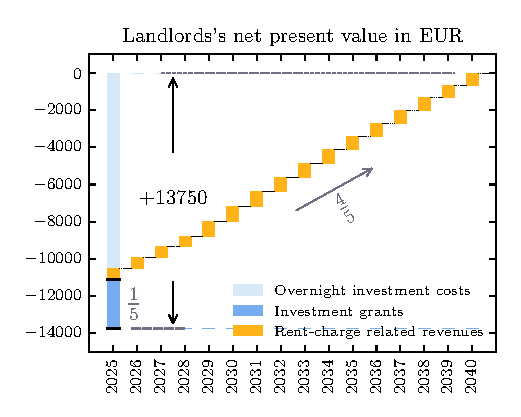
\includegraphics[width=1\linewidth]{figures/3_Methodology/Validate-Landlord.eps}
		\subcaption{Development of property owner's net present value}
		\label{fig:landlord}
	\end{subfigure}
	\begin{subfigure}[c]{0.5\textwidth}
		\centering
		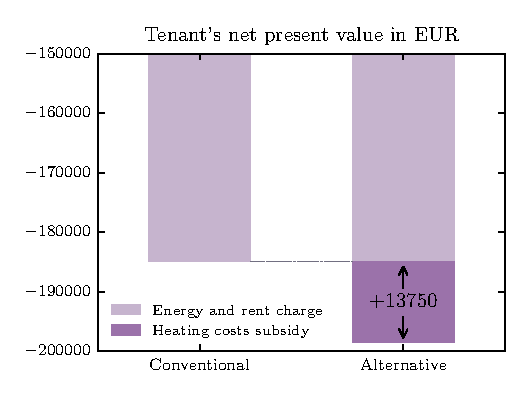
\includegraphics[width=1\linewidth]{figures/3_Methodology/Validate-Tenant.eps}
		\subcaption{Comparison of tenant's net present value}
		\label{fig:tenant}
	\end{subfigure}
	\caption{Property owner's and tenant's net present value and equal financial support. The property owner reaches a net present value equal to zero in 2040 resulting from an investment grant and adjusted rent-charge related revenues. The tenant's net present value remains constant compared to the existing (e.g., gas-fired) heating system due to heating costs subsidy payments.}
	\label{val:npv}
\end{figure}

Until $2040$, both agents receive equal financial support with a total of \SI{13750}{EUR}. One-fifth of the property owner's support is paid as an investment grant directly and four-fifths as rent-charge related revenues from the tenants. The tenant receives a heating costs subsidy. In sum, the governance pays \SI{16500}{EUR}. Thus, the total level of financial support for exchanging the heating system results exactly in (i) a property owner's net present value of cash flows equal to zero within the time horizon of 15 years (see Figure \ref{fig:landlord}) and (ii) a constant remaining net present value of the tenant's energy and rent charges compared with the existing (e.g., gas-fired) heating system (see Figure \ref{fig:tenant}). 

\subsection{Open-source programming environment and data format}\label{met:os}
The developed optimization model is implemented in Python 3.8.12 using the modeling framework Pyomo version 5.7.3 \cite{hart2017optimization}. It is solved with the solver Gurobi version 9.0.3. We use for data analysis the common data format template developed by the Integrated Assessment Modeling Consortium using the open-source Python package pyam \cite{huppmann2021pyam}. Note that all materials used in this study are disclosed as part of the publication at GitHub \footnote{https://github.com/sebastianzwickl}. We refer to the repository for the codebase, data collection, and further information. 